% Options for packages loaded elsewhere
\PassOptionsToPackage{unicode}{hyperref}
\PassOptionsToPackage{hyphens}{url}
%
\documentclass[
]{book}
\usepackage{lmodern}
\usepackage{amssymb,amsmath}
\usepackage{ifxetex,ifluatex}
\ifnum 0\ifxetex 1\fi\ifluatex 1\fi=0 % if pdftex
  \usepackage[T1]{fontenc}
  \usepackage[utf8]{inputenc}
  \usepackage{textcomp} % provide euro and other symbols
\else % if luatex or xetex
  \usepackage{unicode-math}
  \defaultfontfeatures{Scale=MatchLowercase}
  \defaultfontfeatures[\rmfamily]{Ligatures=TeX,Scale=1}
\fi
% Use upquote if available, for straight quotes in verbatim environments
\IfFileExists{upquote.sty}{\usepackage{upquote}}{}
\IfFileExists{microtype.sty}{% use microtype if available
  \usepackage[]{microtype}
  \UseMicrotypeSet[protrusion]{basicmath} % disable protrusion for tt fonts
}{}
\makeatletter
\@ifundefined{KOMAClassName}{% if non-KOMA class
  \IfFileExists{parskip.sty}{%
    \usepackage{parskip}
  }{% else
    \setlength{\parindent}{0pt}
    \setlength{\parskip}{6pt plus 2pt minus 1pt}}
}{% if KOMA class
  \KOMAoptions{parskip=half}}
\makeatother
\usepackage{xcolor}
\IfFileExists{xurl.sty}{\usepackage{xurl}}{} % add URL line breaks if available
\IfFileExists{bookmark.sty}{\usepackage{bookmark}}{\usepackage{hyperref}}
\hypersetup{
  pdftitle={Course manual R programming 2020/2021},
  pdfauthor={Misja Mikkers and Gertjan Verhoeven},
  hidelinks,
  pdfcreator={LaTeX via pandoc}}
\urlstyle{same} % disable monospaced font for URLs
\usepackage{longtable,booktabs}
% Correct order of tables after \paragraph or \subparagraph
\usepackage{etoolbox}
\makeatletter
\patchcmd\longtable{\par}{\if@noskipsec\mbox{}\fi\par}{}{}
\makeatother
% Allow footnotes in longtable head/foot
\IfFileExists{footnotehyper.sty}{\usepackage{footnotehyper}}{\usepackage{footnote}}
\makesavenoteenv{longtable}
\usepackage{graphicx,grffile}
\makeatletter
\def\maxwidth{\ifdim\Gin@nat@width>\linewidth\linewidth\else\Gin@nat@width\fi}
\def\maxheight{\ifdim\Gin@nat@height>\textheight\textheight\else\Gin@nat@height\fi}
\makeatother
% Scale images if necessary, so that they will not overflow the page
% margins by default, and it is still possible to overwrite the defaults
% using explicit options in \includegraphics[width, height, ...]{}
\setkeys{Gin}{width=\maxwidth,height=\maxheight,keepaspectratio}
% Set default figure placement to htbp
\makeatletter
\def\fps@figure{htbp}
\makeatother
\setlength{\emergencystretch}{3em} % prevent overfull lines
\providecommand{\tightlist}{%
  \setlength{\itemsep}{0pt}\setlength{\parskip}{0pt}}
\setcounter{secnumdepth}{5}
\usepackage{booktabs}
\usepackage{amsthm}
\makeatletter
\def\thm@space@setup{%
  \thm@preskip=8pt plus 2pt minus 4pt
  \thm@postskip=\thm@preskip
}
\makeatother
\usepackage[]{natbib}
\bibliographystyle{apalike}

\title{Course manual R programming 2020/2021}
\author{Misja Mikkers and Gertjan Verhoeven}
\date{2021-01-29}

\begin{document}
\maketitle

{
\setcounter{tocdepth}{1}
\tableofcontents
}
\hypertarget{welcome}{%
\chapter*{Welcome}\label{welcome}}
\addcontentsline{toc}{chapter}{Welcome}

This is the website for the course Programming in R at Tilburg University for the course year 2020/2021

\hypertarget{about-this-course}{%
\chapter{About this course}\label{about-this-course}}

\hypertarget{aim-of-the-course}{%
\section{Aim of the course}\label{aim-of-the-course}}

After this course you will be able to import data, manipulate data and to visualize data. In addition you will be able to write (simple) functions to automate (boring) tasks. We will not dive into modeling.

Since visualization is the most interesting part, each lecture is working towards a plot. E.g. in the first lecture, we will start to import (prepared) data and work towards a nice looking graph.

We will teach you to work in Tidyverse. Tidyverse is a package (collection of functions) that is developed to manipulate and visualize data (and more!)

\hypertarget{set-up-of-the-course}{%
\section{Set up of the course}\label{set-up-of-the-course}}

This course is about programming. We believe that the only way to learn programming is by programming yourself. Therefore, we will introduce programming by online programming on the Datacamp website and work in class on notebooks.

Many concepts you will first see at Datacamp and then we apply them in class. Sometimes it will be the other way around: we used something in class and you learn more details about it at Datacamp. This is perfectly fine. However, it is important that you keep up-to-date with Datacamp otherwise you are going to get lost. Also programming is something that you need to practice. You can do the same the Datacamp two or three times. Also the notebooks that we do in class, you can play around with these. Plot different functions, solve equations for different parameter values etc. Just looking at the answers that we give you in class will not help you to learn programming.

Finally, we urge you to use google (or other search engines like DuckDuckGo) and stackoverflow with your assignments. Some students find this weird at the beginning: should we not teach you everything that you need to know? The answer is ``no'', for a number of reasons. First, even professional programmers use google and stackoverflow all the time. Second, python and R are open source and lots of people work with it. If you encounter a problem, chances are that someone else had the same problem and knows the solution to it. There is not need to ``invent the wheel''. Use the resources available to you. If you copy a lot of code, you should add a reference. Finally, because python and R are open source, they develop rapidly. The things that we teach you now, will be obsolete in a couple of years time. Hence, you need to be able to find your way around also in 10 years time. It will help you a lot to specifically google your error messages.
To start practicing this, use google now.

\hypertarget{questions}{%
\section{Questions}\label{questions}}

here are no stupid questions, it's stupid not to ask questions. We encourage you to post your questions in the discussion section on Canvas.

Only when you need to include privately sensitive information (``my cat has passed away''), you can send an email. Always provide us with the following information: - say whether you are an ECO or EBE student - mention the group number of your tutorial and/or the name of your tutorial teacher - explain your question

\hypertarget{team}{%
\section{Team}\label{team}}

The R-part of the course Programming for Economists in 2020-2021 is taught by:

\begin{itemize}
\tightlist
\item
  José Carreño Bustos
\item
  Misja Mikkers
\item
  Daan Schrage
\item
  Gertjan Verhoeven
\item
  Jierui Yang
\end{itemize}

\hypertarget{exam}{%
\section{Exam}\label{exam}}

This year the midterm exam will be a an exam with multiple choice questions and ``closed'' questions (e.g.~you have to give a number). You can use R-studio on your own computer and you are allowed to google. You are not allowed to communicatie with other people.

The midterm exam will last for one hour and will consist of 10 questions about github, markdown and R. Once you answer a question and go on to the next question, you cannot go back to an earlier question.

We will not provide a test-exam. The notebooks used in class show the kind of questions we will ask you.

\hypertarget{schedule}{%
\chapter{Schedule}\label{schedule}}

\hypertarget{lecture-1-visualisation}{%
\section{Lecture 1: Visualisation}\label{lecture-1-visualisation}}

\hypertarget{week-8}{%
\subsection{Week 8}\label{week-8}}

February 22, 2021 - February 26, 2021

\hypertarget{preparation}{%
\subsection{Preparation}\label{preparation}}

Before class you should have

\begin{itemize}
\tightlist
\item
  installed the software
\item
  cloned the repo from\url{https://github.com/misjamikkers/Rprogramming21_student} on your computer
\item
  finished datacamp course ``Introduction to the Tidyverse''
\end{itemize}

\hypertarget{in-class}{%
\subsection{In class}\label{in-class}}

In class we will go through the notebook of lecture 1

\hypertarget{lecture-2-data-wrangling-1}{%
\section{Lecture 2: Data wrangling 1}\label{lecture-2-data-wrangling-1}}

\hypertarget{week-9}{%
\subsection{Week 9}\label{week-9}}

March 1, 2021 - March 5, 2021

\hypertarget{preparation-1}{%
\subsection{Preparation}\label{preparation-1}}

Before class you should have

\begin{itemize}
\tightlist
\item
  finished datacamp course ``Introduction to R''
\end{itemize}

\hypertarget{in-class-1}{%
\subsection{In class}\label{in-class-1}}

In class we will go through the notebook of lecture 2

\hypertarget{lecture-3-data-wrangling-2}{%
\section{Lecture 3: Data wrangling 2}\label{lecture-3-data-wrangling-2}}

\hypertarget{week-10}{%
\subsection{Week 10}\label{week-10}}

March 8, 2021 - March 12, 2021

\hypertarget{preparation-2}{%
\subsection{Preparation}\label{preparation-2}}

\begin{itemize}
\tightlist
\item
  downloaded some data
\item
  made your own notebook with some data wrangling and a plot
\end{itemize}

The aim of this preparation is to practice with the skills required until now. This should be a good preparation for the exam with respect to the basis programming skills.

\hypertarget{in-class-2}{%
\subsection{In class}\label{in-class-2}}

In class we will have some time to answer your questions with respect to your prepared notebook.

Furthermore, we will go through the notebook of lecture 3.

\hypertarget{lecture-4-functions-and-r-markdown}{%
\section{Lecture 4: Functions and R Markdown}\label{lecture-4-functions-and-r-markdown}}

\hypertarget{week-11}{%
\subsection{Week 11}\label{week-11}}

March 15, 2021 - March 19 2021

\hypertarget{preparation-3}{%
\subsection{Preparation}\label{preparation-3}}

For a super compact introduction to R Markdown, watch \href{https://vimeo.com/178485416}{This 1-minute video}.

Got that? No worries, we go over it step by step in the R notebooks.

``A reproducible workflow'' by Ignasi Bartomeus and Francisco Rodríguez-Sánchez (\url{https://youtu.be/s3JldKoA0zw}) is a 2-min video that looks artistic but also shows very common and practical problems in data analysis, and how R markdown solves these.

\hypertarget{in-class-3}{%
\subsection{In class}\label{in-class-3}}

In class we will go through the notebooks of lecture 4.
First is the functions notebook, then the R Markdown notebook (that includes a Markdown refresher notebook as exercise).

\hypertarget{lecture-5-generating-data-and-some-statistics}{%
\section{Lecture 5: Generating data and some statistics}\label{lecture-5-generating-data-and-some-statistics}}

\hypertarget{week-12}{%
\subsection{Week 12}\label{week-12}}

March 22, 2021 - March 26, 2021

\hypertarget{preparation-4}{%
\subsection{Preparation}\label{preparation-4}}

Nothing.

\hypertarget{in-class-4}{%
\subsection{In class}\label{in-class-4}}

In class we will go through the notebook of lecture 5.

\hypertarget{installing-the-software}{%
\chapter{Installing the software}\label{installing-the-software}}

Rstudio provides a good \href{https://education.rstudio.com/learn/beginner/}{starting point for beginners} to learn R and Rstudio.

In particular, the first chapter of moderndive and the first chapter of R for data science.

\hypertarget{what-do-you-need}{%
\section{What do you need?}\label{what-do-you-need}}

We assume you have a laptop (Windows or Mac). To be able to follow the course and use the software for other courses you need the following free software:

\begin{itemize}
\tightlist
\item
  R
\item
  Rstudio
\item
  TinyTex
\item
  R packages
\end{itemize}

R is free software for importing data, manipulating data and statistical analysis. Once installed, you don't need to open the software.

We will use R in another program: Rstudio. Rstudio is a so called Integrated Development Environment (IDE), which allows you to write and run code.

Rstudio is able to transform your code to different nice outputs:

\begin{itemize}
\tightlist
\item
  notebook
\item
  presentation
\item
  article
\item
  thesis
\item
  much more (even this website and this course manual is build in Rstudio!)
\end{itemize}

Rstudio needs TinyTex to transform your code to pdf (which is our preferred format, however other formats are also possible).

If you need to do things more often, it is useful to write a function to do these things. Other R users also use functions and store them in packages. Some of these packages are published online and can be used by all users. We will depend in our course on some of these packages.

The first package we will install is the package TinyTex, which is basically a function to install the TinyTex software on your computer, taking into account your operating system.

We also show you how to install other packages.

In this chapter we will instruct how to install the software.

\hypertarget{installing-r}{%
\section{Installing R}\label{installing-r}}

In this paragraph we will take you through the steps to install R.

\begin{enumerate}
\def\labelenumi{\arabic{enumi}.}
\tightlist
\item
  Go to this \href{https://mirror.lyrahosting.com/CRAN/}{website}
\item
  Choose download R for your operating system. You can choose from Windows, Mac OS X for apple computers and Linux. If you don't know which operating system you have and you don't have an apple computer, you may guess you have a Windows computer.
\item
  After downloading, open the downloaded file and follow the steps to install the program. Choose the default options.
\end{enumerate}

\hypertarget{r-studio}{%
\section{R studio}\label{r-studio}}

You can download and install R studio from \url{http://www.rstudio.com/download}. Choose the option: ``Open Source License Free''. The website will then recommend a version for your operating system.

You will see 3 ``panes'':

\begin{enumerate}
\def\labelenumi{\arabic{enumi}.}
\tightlist
\item
  Console (left part of the screen)
\item
  Environment/history etc (top right of your screen)
\item
  Files/Plots/Packages (bottom right of your sreen)
\end{enumerate}

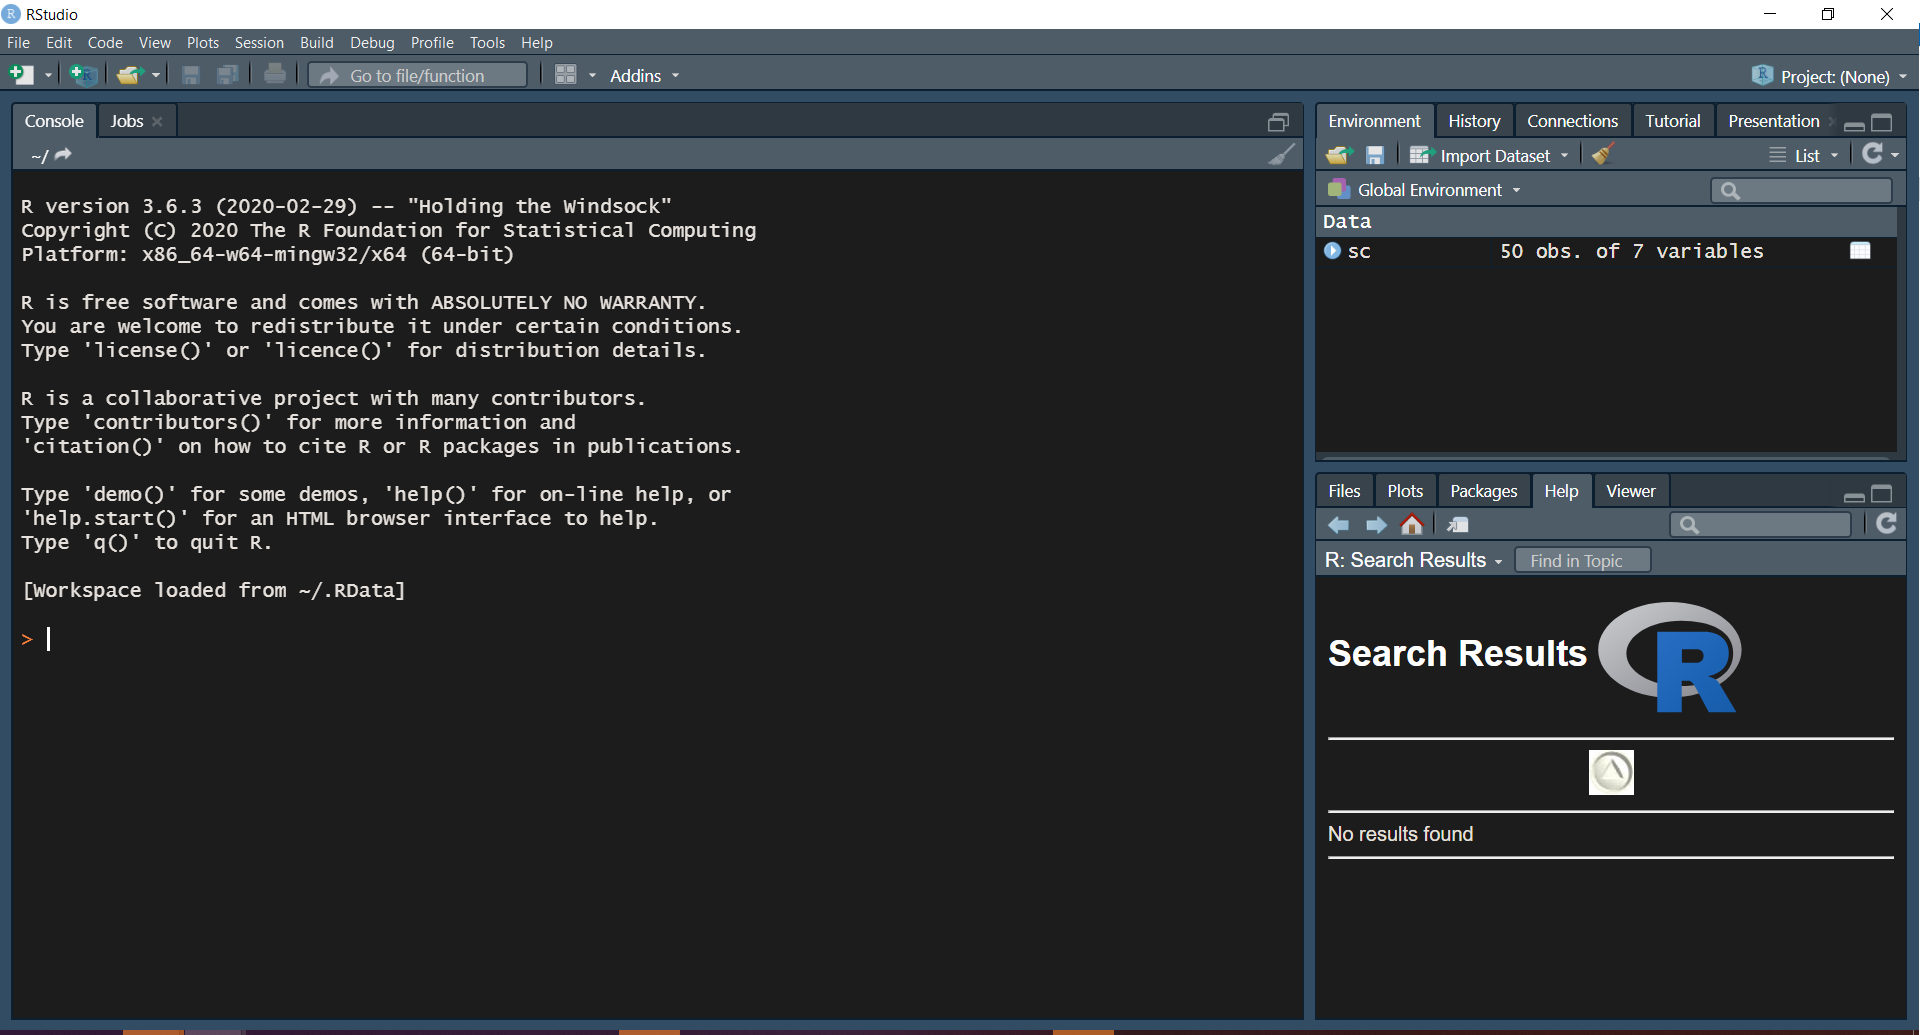
\includegraphics{Rstudio.PNG}

You can test the installation by typing

1 + 1

followed by an enter to test the installation.

\hypertarget{installation-of-tinytex}{%
\section{Installation of TinyTex}\label{installation-of-tinytex}}

LaTeX is a commonly used open source typesetting system; it includes features designed for the production of technical and scientific documentation. LaTeX is the used often in preparing scientific documents.
Latex and R-studio can work together. So you can transform your Rmd documents to pdf via the ``knit'' button.
TinyTex is a Latex distribution that works on MAC, Windows and Linux operating systems.

We have to install TinyTex in 2 steps:

Run this command in your console (button at the left bottom of your screen)

\begin{itemize}
\tightlist
\item
  Step 1
\end{itemize}

install.packages(`tinytex')
tinytex::install\_tinytex()

\begin{itemize}
\tightlist
\item
  Step 2
\end{itemize}

writeLines(c(
`\textbackslash documentclass\{article\}',
`\textbackslash begin\{document\}', `Hello world!', `\textbackslash end\{document\}'
), `test.tex')
tinytex::pdflatex(`test.tex')

\hypertarget{installation-of-packages}{%
\section{Installation of packages}\label{installation-of-packages}}

In the pane at the bottom right there is a tab called ``Packages'' (see screenshot above).
After clicking this tab a new tab ``Install'' appears

After clicking the ``Install'' button, you can type tidyverse in the pop-up.

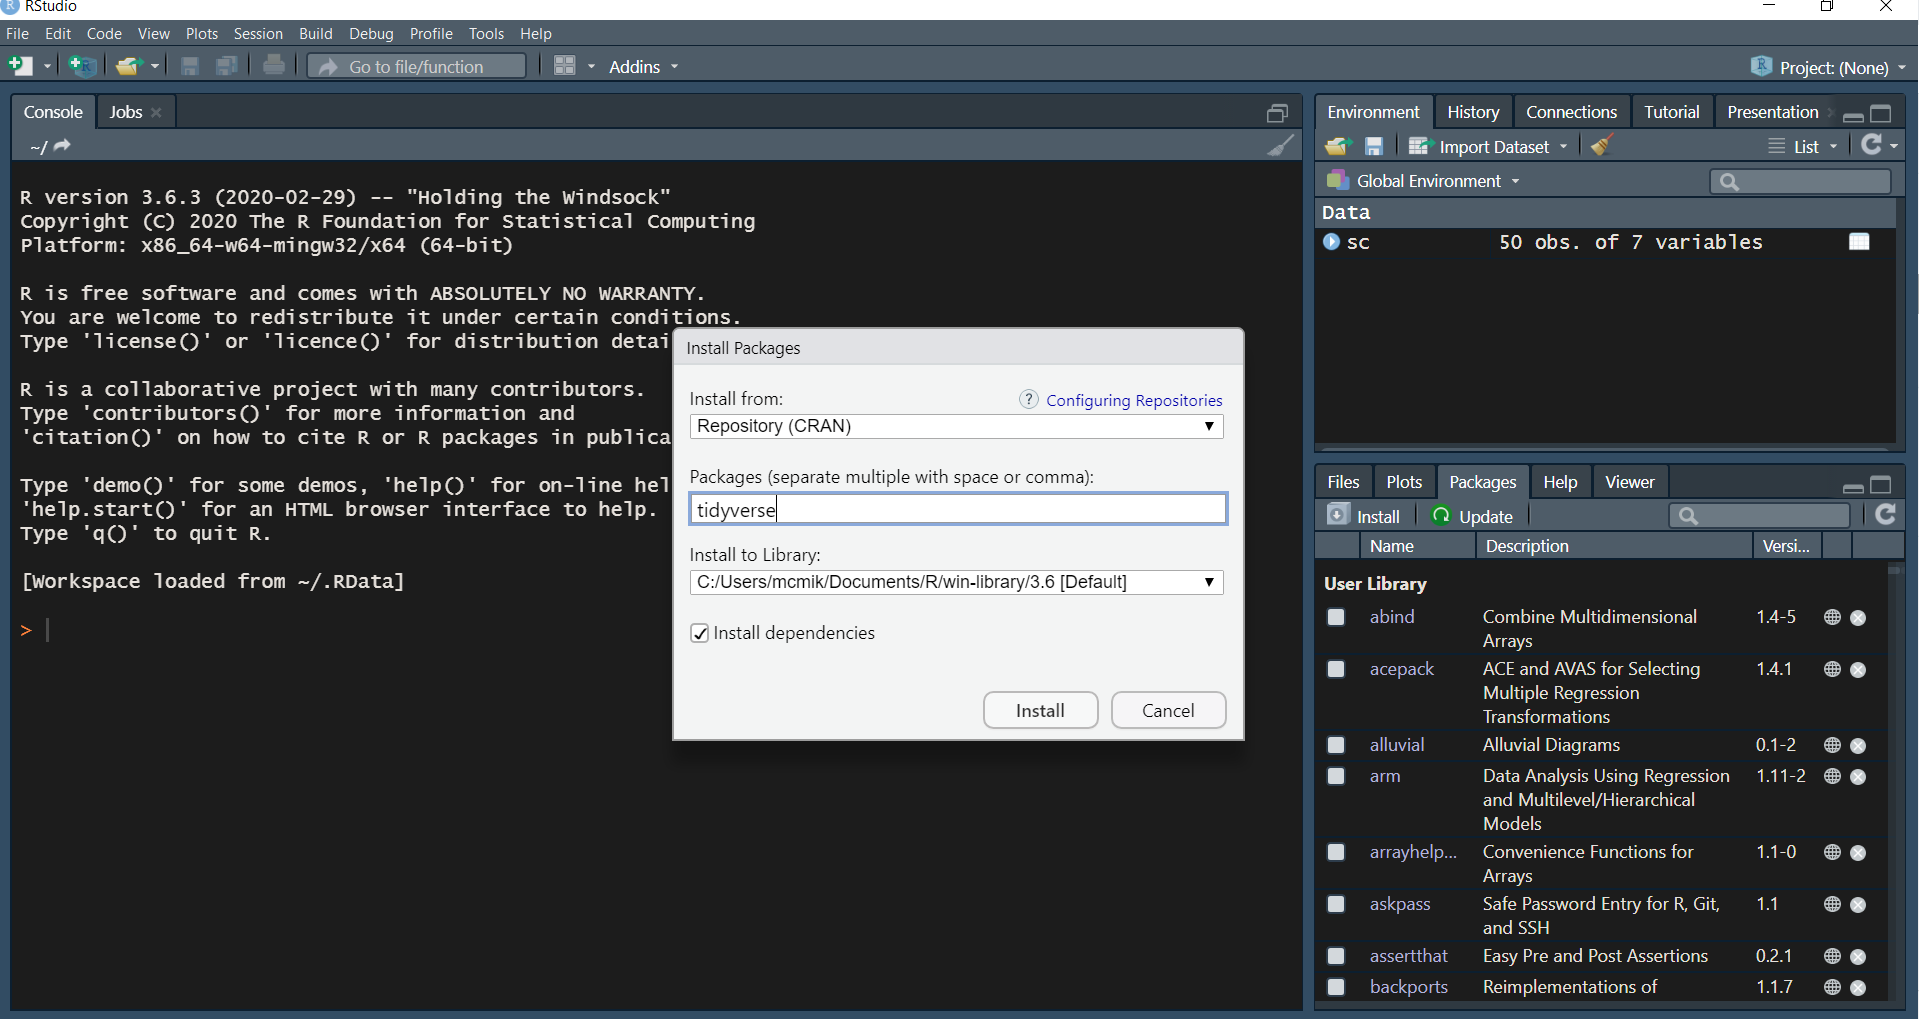
\includegraphics{install.PNG}

Please install the package tidyverse.

  \bibliography{book.bib,packages.bib}

\end{document}
